% Standalone manuscript: upload this .tex file to Overleaf and use pdfLaTeX.
% All references, proofs and the analytical figure are contained here.
\documentclass[11pt,a4paper]{article}
\usepackage[margin=25mm]{geometry}
\usepackage[T1]{fontenc}
\usepackage{lmodern,microtype,amsmath,amssymb,amsthm,booktabs,tabularx}
\usepackage{tikz}
\usepackage[colorlinks=true,linkcolor=blue,citecolor=blue,urlcolor=blue]{hyperref}
\usepackage{bookmark}
\newtheorem{theorem}{Theorem}[section]
\newtheorem{proposition}[theorem]{Proposition}
\newtheorem{corollary}[theorem]{Corollary}
\newcommand{\ind}{\mathbf{1}}
\newcommand{\cwnd}{\mathrm{cwnd}}
\newcommand{\gcrit}{g_{\mathrm c}}
\setlength{\emergencystretch}{2em}
\numberwithin{equation}{section}
\title{Pacing and Congestion-Window Growth:\\An Exact Packet-Level Analysis}
\author{Skai Uijing}
\date{October 8, 2026}
\begin{document}
\maketitle

\begin{abstract}
An unchanged per-ACK window update can produce different growth in physical
time when newly available window credit passes through a pacer. We study this
effect in a loss-free, fixed-delay packet model: each slow-start ACK reserves
two packets, their spacing is set by the updated window and a fixed gain, and
existing reservations retain their timestamps. We solve the transmission
recurrence exactly for every gain $g\ge1$. A fixed-batch comparator supplies a
Fibonacci lower bound, while immediate transmission supplies the doubling
upper bound. The exact solution identifies a transition at $g=2\ln2$: below
it, additional ACK waiting ends after a finite prefix; above it, each RTT
contains a sending interval followed by persistent waiting. The sending span
approaches $(2\ln2/g)R$, and the normalized window growth exponent is
$\min\{g/2,\ln2\}$. Packet timestamps converge to those of the immediate-send
model as gain tends to infinity. For loss-free congestion avoidance, we derive
an exact event recurrence and a queue-clock decomposition with a logarithmic
term, leaving the cumulative ACK-waiting contribution explicit. All results
concern the specified scheduler; no equivalence to a deployed TCP stack or
network-performance improvement is assumed.
\end{abstract}

\section{The timing question}
This work began while developing SCP, a TCP-like transport with a Reno-like
controller. Replacing burst sending with pacing made transfers slower in the
author's development runs, despite little change in the useful-data fraction.
That observation motivated a narrower mathematical question: with the window
update held fixed, how does transmission scheduling change the times at which
ACKs return and the window grows? The observation is motivation, rather than
evidence that the model below explains the full implementation's performance.

Consider a one-packet initial window. Send that packet at time zero. Its ACK
returns at $R$ and raises the window to two packets. If the next two packets
leave at $R$ and $1.5R$, only the first has been acknowledged at $2R$: the
window is three, not four. The window was updated immediately at each ACK.
The difference comes from transmission times, not from postponing window
updates to RTT boundaries.

The analysis follows three steps. We first specify a packet scheduler and
separate actual flight from future reservations. We then compare its growth
with two solvable extremes, before obtaining its exact transmission times
for general pacing gain. Finally, we carry the same event accounting into
congestion avoidance. The main object is $\cwnd(t)$ and its underlying packet
trace, not an optimization of network throughput or a replacement congestion
controller.

\section{Model and event accounting}\label{sec:model}
\subsection{Assumptions and units}
Every packet has payload size $M$, and its ACK returns exactly $R>0$ after
actual transmission. There is no loss, reordering, ACK aggregation, application
limitation, receiver-window limitation, or link-serialization constraint.
These assumptions isolate feedback timing. In particular, an instantaneous
burst is an admissible comparison trace in this ideal model.

Write $\tau=t/R$ and $w(\tau)=\cwnd(R\tau)/M$. All timestamps below are in
units of $R$, and windows and packet counts are in units of $M$. The initial
window is one packet; packet 0 is sent at $s_0=0$. During the slow-start
analysis, the connection remains in slow start indefinitely and every ACK
increases $w$ by one. This is the full-packet, one-ACK-per-packet specialization
of the slow-start update; Section~\ref{sec:ca} treats a finite threshold and
the real-valued congestion-avoidance update \cite{rfc5681}.

At a shared timestamp, process ACKs before transmissions and sample after all
events there. Sampling at integer $\tau$ does not change the event schedule.
The gain $g\ge1$ is fixed. Notation used throughout is collected in
Table~\ref{tab:notation}.

\begin{table}[htbp]
\centering\small
\caption{Notation. Physical timestamps equal normalized timestamps times $R$.}
\label{tab:notation}
\begin{tabularx}{\linewidth}{@{}lX@{}}\toprule
Symbol & Meaning\\\midrule
$F,Q$ & Sent but unacknowledged packets; reserved but unsent packets\\
$s_j$ & Actual send time of packet $j$, numbered from zero\\
$a_k,w_k$ & Arrival time of ACK $k$, and window immediately after it\\
$b_k,T_k$ & First send in ACK $k$'s batch; next free slot after that batch\\
$N_g(\tau)$ & Number of actual transmissions by $\tau$, including packet 0\\
$H_k$ & $\sum_{r=1}^k1/r$, with $H_0=0$\\
$D(j)$ & $H_{2j}-H_j$; a harmonic sum, not a traffic counter\\
$B_m$ & $b_{2^m}$, the first send associated with an ACK-index block\\
$f_n$ & Fibonacci numbers, $f_0=0$, $f_1=1$\\\bottomrule
\end{tabularx}
\end{table}

\subsection{Window credit and the append rule}
After each reservation step, the scheduler maintains
\begin{equation}
 F+Q=w.\label{eq:invariant}
\end{equation}
An actual transmission transfers one packet from $Q$ to $F$, preserving the
sum. An ACK reduces $F$ by one and increases $w$ by one, creating exactly two
new reservation positions. Reserving two packets restores
\eqref{eq:invariant}. Hence $F\le w$ at every transmission, and queued packets
cannot consume the same credit twice.

After ACK $k$, $w_k=k+1$. The two new packets are appended after every existing
reservation, with spacing $1/[g(k+1)]$. Existing timestamps remain unchanged.
The scheduler also retains one spacing after the last packet of each batch.
With $T_0=1/g$, its complete recurrence is
\begin{align}
 a_k&=s_{k-1}+1,& b_k&=\max\{a_k,T_{k-1}\},\label{eq:ack}\\
 s_{2k-1}&=b_k,&s_{2k}&=b_k+\frac1{g(k+1)},\label{eq:sends}\\
 T_k&=b_k+\frac2{g(k+1)}.&&\label{eq:tail}
\end{align}
Here $T$ is the next free slot after the \emph{entire} queue, even when that
queue is long. The rate is selected at reservation time. It is not recalculated
at the eventual transmission of an already reserved packet. This distinction
is part of the model, not a consequence of specifying $g\cwnd/R$ alone.

Packet sends are strictly ordered for finite $g$. The fixed feedback delay
therefore preserves their order, justifying $a_k=s_{k-1}+1$. Each reservation
is causal because $b_k\ge a_k$. Also, $b_1=1$, and for $k\ge2$,
\begin{equation}
 b_k=\max\left\{a_k,b_{k-1}+\frac2{gk}\right\}.\label{eq:max}
\end{equation}
In particular, the ACK branch can be written without packet timestamps:
\begin{equation}
 a_{2j}=b_j+1,\qquad
 a_{2j+1}=b_j+1+\frac1{g(j+1)}\quad(j\ge1).\label{eq:parents}
\end{equation}

\subsection{From actual transmissions to the window}
Equation~\eqref{eq:max} implies $b_k\ge1+(2/g)(H_k-1)\to\infty$,
so only finitely many packets leave in any finite time interval.
Set $N_g(x)=0$ for $x<0$. For $x\ge0$, count actual sends, not reservations:
\begin{equation}
 N_g(x)=1+\sum_{k\ge1}\left(
 \ind_{\{b_k\le x\}}+
 \ind_{\{b_k+1/[g(k+1)]\le x\}}\right).
\end{equation}
The slow-start window is exactly
\begin{equation}
 \boxed{w_g(\tau)=1+N_g(\tau-1).}\label{eq:count}
\end{equation}
Gain changes the times of ACKs, not the window $k+1$ after ACK $k$.

For integer samples, write $W_n=w_g(n)$ and let $S_n$ count sends in
$(n,n+1]$. Those packets are acknowledged in $(n+1,n+2]$, so
\begin{equation}
 \boxed{W_{n+2}=W_{n+1}+S_n.}\label{eq:conservation}
\end{equation}
This identity is shared by the comparison models below. It neither assumes
RTT-batched ACK processing nor determines $S_n$ without a scheduling rule.

\section{Two comparison models}\label{sec:comparison}
\subsection{Immediate transmission gives the upper bound}
For any sender satisfying these slow-start assumptions and the flight
constraint, the ACKs in $(n,n+1]$ can only come from packets in flight just
after $n$. A packet sent strictly after $n$ is acknowledged strictly after
$n+1$. Each returning ACK adds one window unit, hence
\begin{equation}
 W_{n+1}-W_n\le F(n)\le W_n.
\end{equation}
Since $W_0=1$, induction gives $W_n\le2^n$. The sender that immediately sends
both newly permitted packets at every ACK attains this bound. Its physical
window at the boundaries is
\begin{equation}
 \cwnd_{\mathrm{burst}}(nR)=M2^n.\label{eq:upper}
\end{equation}
This is a timing bound in a fixed-delay, unlimited-service model, not a claim
that burst sending maximizes throughput on a congested network.

\subsection{A fixed-batch comparator gives Fibonacci growth}
Define a separate sender that reads its window $\widehat W_n$ at each integer time $n$
after ACK processing, and sends $\widehat W_n$ packets at
\begin{equation}
 n+\frac{i}{\widehat W_n},\qquad i=0,\ldots,\widehat W_n-1.\label{eq:fixed}
\end{equation}
ACKs still increase its window immediately, but do not change the current
batch. In $(n,n+1]$ there are $\widehat W_n-1$ remaining packets of this batch and the
first packet of the next batch. Equation~\eqref{eq:conservation} gives
\begin{equation}
 \widehat W_{n+2}=\widehat W_{n+1}+\widehat W_n,\quad
 \widehat W_0=1,\quad \widehat W_1=2,
 \qquad \widehat W_n=f_{n+2}.\label{eq:fib}
\end{equation}
Its window sequence is $1,2,3,5,8,13,\ldots$. Its explicit boundary formula is
\begin{equation}
 \cwnd_{\mathrm{fixed}}(nR)
 =\frac{M}{\sqrt5}(\phi^{n+2}-\psi^{n+2}),\qquad
 \phi=\frac{1+\sqrt5}{2},\quad\psi=\frac{1-\sqrt5}{2}.\label{eq:binet}
\end{equation}
The sender respects the actual-flight limit. Indeed, in a batch with previous
size $p=f_{n+1}$ and current size $q=f_{n+2}$, its flight just after phase
$0\le u<1$ is $p+\lfloor qu\rfloor-\lfloor pu\rfloor\le q$, while its
window is at least $q$. Unlike the append scheduler, it permits future plans
to rely on future flight releases; it does not enforce the same reservation
invariant $F+Q=w$ at planning time.

Solving this comparator alone does not make it a lower bound. The needed
comparison is between \emph{actual} send times.
\begin{theorem}[Fibonacci-to-doubling sandwich]\label{thm:sandwich}
For the append scheduler of Section~\ref{sec:model}, every fixed $g\ge1$
satisfies, for integers $n\ge0$,
\begin{equation}
 \boxed{Mf_{n+2}\le\cwnd_g(nR)\le M2^n.}\label{eq:sandwich}
\end{equation}
\end{theorem}
The upper bound was proved above. Appendix~\ref{app:fib} proves that at $g=1$
each packet leaves no later than its fixed-batch counterpart. Fixed feedback
delay then preserves the ordering of ACKs and windows. The gain monotonicity
proved in Section~\ref{sec:limit} extends the lower bound to $g\ge1$.
The comparison is not justified merely by reserving packets earlier, and it
does not assert the local service condition $S_n\ge W_n$ for arbitrary pacers.

\section{Exact transmission times for every gain}\label{sec:exact}
Let $c=2/g$ and $D(j)=H_{2j}-H_j$. Two elementary facts will identify which
branch of \eqref{eq:max} is active:
\begin{equation}
 D(j+1)-D(j)=\frac1{(2j+1)(2j+2)}>0,\qquad
 D(j)<\ln2,\qquad D(j)\longrightarrow\ln2.\label{eq:harmonic}
\end{equation}
The inequality follows by comparing the sum with $\int_j^{2j}dx/x$; the limit
follows from $H_j=\ln j+\gamma_E+O(1/j)$, where $\gamma_E$ is Euler's constant.

Group ACK indices as $q\le k<2q$, where $q=2^m$, and write $B_m=b_{2^m}$.
These groups are analytical partitions of the event indices. The sender does
not wait for a group or an RTT boundary to process an ACK.

\begin{theorem}[Unified exact solution]\label{thm:exact}
For every fixed $g\ge1$,
\begin{align}
 B_0&=1,&
 B_{m+1}&=B_m+\max\{1,cD(2^m)\},\label{eq:block}\\
 b_k&=B_m+c(H_k-H_{2^m}),&&2^m\le k<2^{m+1}.\label{eq:within}
\end{align}
Equivalently, with $[x]_+=\max(x,0)$ and an empty sum equal to zero,
\begin{equation}
 \boxed{b_k=cH_k+1-c+
 \sum_{i=0}^{\lfloor\log_2k\rfloor-1}[1-cD(2^i)]_+.}\label{eq:closed}
\end{equation}
Together with \eqref{eq:sends}, this determines every packet timestamp.
\end{theorem}

\begin{proof}
The first group contains only $k=1$, for which $b_1=1$. Assume the formulas
hold before a group with $q=2^m$, $m\ge1$. At its first index,
\begin{align*}
 a_q&=b_{q/2}+1=B_{m-1}+1,\\
 T_{q-1}&=b_{q-1}+c/q=B_{m-1}+c(H_q-H_{q/2}).
\end{align*}
Their maximum proves the formula for $B_m$. Set
$\Delta=B_m-B_{m-1}\ge1$.

Within this group, proceed in increasing $k$. For an even $k=2j>q$, the
already established formulas give
\begin{equation}
 T_{2j-1}-a_{2j}
 =\Delta-1+c[D(j)-D(q/2)]>0.\label{eq:even}
\end{equation}
Here $q/2<j<q$, and $D$ strictly increases. For an odd $k=2j+1>q$,
\begin{equation}
 \begin{split}
 T_{2j}-a_{2j+1}
 =\Delta-1+c\left[D(j)-D(q/2)
          +\frac1{2j+1}-\frac1{2j+2}\right]>0.
 \end{split}\label{eq:odd}
\end{equation}
The last difference is positive even when $j=q/2$. Thus every interior step
selects the queue-tail branch of \eqref{eq:max}. Summing $c/k$ from the group
start proves \eqref{eq:within} and completes strong induction.

Finally expand \eqref{eq:block}, use $\max(1,x)=x+[1-x]_+$ and telescope
$\sum_{i<m}D(2^i)=H_{2^m}-1$ to obtain \eqref{eq:closed}.
\end{proof}

The proof also identifies all possible extra waiting: apart from the initial
ACK, it can occur only at ACK indices $2^m$. This conclusion follows from the
two branches of the actual recurrence, rather than an assumption that the
pacer stays busy.

\section{Sending spans, waiting, and the gain transition}\label{sec:span}
\subsection{Finite-group formulas}
Group $m$, with $q=2^m$, consists of $q$ two-packet batches. Its $2q$ packets
have indices $2q-1,\ldots,4q-2$. The first leaves at $B_m$; the last leaves at
\begin{equation}
 s_{4q-2}=b_{2q-1}+\frac1{2gq}
         =B_m+\frac2gD(q)-\frac1{2gq}.
\end{equation}
Let $L_m$ be the physical time from that first send to that last send.
Let $I_m$ be the extra wait between the final reserved slot of this group and
the start of the next, and let $G_m$ be the actual last-to-next-first gap.
Then
\begin{equation}
 \boxed{\begin{aligned}
 L_m/R&=\frac2gD(q)-\frac1{2gq},\\
 I_m/R&=\left[1-\frac2gD(q)\right]_+,\\
 G_m/R&=I_m/R+\frac1{2gq}.
 \end{aligned}}\label{eq:span}
\end{equation}
The first line is a timestamp span, not link busy time. The second excludes
the nominal last-packet spacing. The third includes that spacing.

An extra wait occurs after this finite group exactly when
\begin{equation}
 g>g_m:=2D(2^m).\label{eq:finitecritical}
\end{equation}
The first thresholds are $g_0=1$, $g_1=7/6$, and $g_2=533/420$.
They increase to $2\ln2$. Thus gains below the limiting threshold can still
produce waiting during a finite initial part of the trace.

\subsection{The three limiting regimes}
\begin{corollary}[Transition at $\gcrit=2\ln2$]\label{cor:transition}
For $1\le g<\gcrit$, additional ACK waiting ends after finitely many groups.
For $g=\gcrit$, every group has a positive additional wait, but its length
tends to zero. For $g>\gcrit$, the additional wait tends to the positive
fraction $1-\gcrit/g$ of an RTT.
\end{corollary}
\begin{proof}
Use $D(2^m)\uparrow\ln2$ in \eqref{eq:block} and \eqref{eq:span}. If
$g<\gcrit$, then $cD(2^m)>1$ eventually, so $I_m=0$ thereafter. Equations
\eqref{eq:even}--\eqref{eq:odd} exclude additional waiting inside each group.
If $g\ge\gcrit$, then $cD(2^m)<1$ for every finite $m$, so $B_m=m+1$ and
$I_m/R=1-cD(2^m)$, with the stated limits.
\end{proof}

Below the threshold, the inter-group duration tends to
$2\ln2/g>1$ in RTT units. These index groups may span more than an RTT, but
their separating gaps tend to zero. Thus they do not form persistent
RTT-separated bursts. Indeed the eventual consecutive packet spacings are
$1/[g(k+1)]$, repeated twice, and decrease to zero; a fixed RTT observation
interval has first-to-last send span tending to $R$.

At and above the threshold, group $m$ starts at $(m+1)R$ and ends before
$(m+2)R$. Only in this regime can its span be identified directly with the
span of the packets in that integer RTT. Equation~\eqref{eq:span} gives
\begin{equation}
 \boxed{\lim_{m\to\infty}L_m/R=\frac{2\ln2}{g},\qquad
 \lim_{m\to\infty}I_m/R=1-\frac{2\ln2}{g}.}\label{eq:spanlimit}
\end{equation}
For $g=2$ the limiting sending span is $\ln2\simeq0.69315$ RTT; for $g=4$
it is about $0.34657$ RTT. A regular local pacing interval therefore does not
prevent global concentration: the sender finishes its available packets
earlier and then waits for feedback. The proof of this statement is the exact
recurrence, not the heuristic integral $\int_W^{2W}2\,dx/(gx)$.

\section{Window growth in physical time}\label{sec:growth}
\subsection{Below the threshold: exponent and amplitude}
For $g<\gcrit$, the positive-part sum in \eqref{eq:closed} eventually stops
changing. Define the finite sum
\begin{equation}
 \delta_g=1-c+\sum_{i\ge0}[1-cD(2^i)]_+.
\end{equation}
For every sufficiently large $k$, the equality $b_k=cH_k+\delta_g$ is exact.
Both packets in batch $k$ consequently have times
$c\ln k+c\gamma_E+\delta_g+O(1/k)$. Inverting this relation changes the
corresponding batch count by only $O(1)$, and there are two packets per batch.
Therefore
\begin{align}
 N_g(\tau)&=2e^{(\tau-\delta_g)/c-\gamma_E}+O(1),\\
 w_g(\tau)&=A_g e^{g\tau/2}+O(1),\qquad
 A_g=2e^{-(1+\delta_g)/c-\gamma_E}>0.\label{eq:lowgrowth}
\end{align}
The second line uses the exact one-RTT shift in \eqref{eq:count}.

For $g=1$, $c=2$ and $2D(2^i)\ge1$, so $\delta_1=-1$. In fact, for all
$k\ge1$,
\begin{equation}
 b_k=2H_k-1,\qquad
 w_1(\tau)=2e^{\tau/2-\gamma_E}+O(1).\label{eq:unity}
\end{equation}
The asymptotic multiplier per RTT is $\sqrt e$. It exceeds the Fibonacci
multiplier $\phi$, but is smaller than the immediate-send multiplier 2.

\subsection{At and above the threshold: the within-RTT trajectory}
When $g\ge\gcrit$, the exact solution reduces to
\begin{equation}
 b_k=m+1+\frac2g(H_k-H_{2^m}),\qquad 2^m\le k<2^{m+1}.\label{eq:high}
\end{equation}
For $n\ge2$, ACK $2^{n-1}$ arrives at $n$ because
$a_{2^{n-1}}=b_{2^{n-2}}+1=n$; the next ACK arrives later. The case $n=1$
follows from the initial packet. Thus every finite $g\ge\gcrit$ has the same
integer-boundary window:
\begin{equation}
 \boxed{w_g(n)=1+2^{n-1}\quad(n\ge1).}\label{eq:boundary}
\end{equation}
The trajectories between those boundaries are different.

To see their shape, let $P_{n,g}(u)$ be the fraction of packets in
$[n,n+1)$ that have been sent by $n+u$, $0\le u<1$; set $P_{n,g}(1)=1$.
For high gain the interval contains $2^n=2q$ packets, where $q=2^{n-1}$.
Uniformly for $q\le k<2q$,
\begin{equation}
 b_k-n=\frac2g\ln(k/q)+O_g(1/q).
\end{equation}
Hence the number of batches reached by phase $u$ is
$q\min\{e^{gu/2}-1,1\}+O_g(1)$. Counting two packets per batch gives
\begin{equation}
 P_{n,g}(u)\longrightarrow\min\{e^{gu/2}-1,1\}.\label{eq:highcdf}
\end{equation}
The endpoint error affects at most $O_g(1)$ packets. The previous round's
packets provide the present round's ACKs, so \eqref{eq:count} yields
\begin{equation}
 \boxed{w_g(n+u)=2^{n-1}\min\{e^{gu/2},2\}+O_g(1),\quad0\le u<1.}
 \label{eq:phase}
\end{equation}
For fixed finite $g$, the error can be bounded uniformly in $u$. At
$g=\gcrit$, this simplifies to $w_g(\tau)=2^{\tau-1}+O(1)$. Above the
threshold, growth followed by a plateau persists within each RTT; one
constant times $2^\tau$ does not describe all phases with relative error
tending to zero.

For comparison, \eqref{eq:lowgrowth} gives the lower-gain send distribution
by taking differences of cumulative sends at the endpoints:
\begin{equation}
 P_{n,g}(u)\longrightarrow
 \frac{e^{gu/2}-1}{e^{g/2}-1},\qquad1\le g<\gcrit.\label{eq:lowcdf}
\end{equation}
The two limits agree at $\gcrit$. They describe the fraction of this RTT's
packets sent, not the normalized window. Figure~\ref{fig:phase} plots the
high-gain expression directly.

\begin{figure}[htbp]
\centering
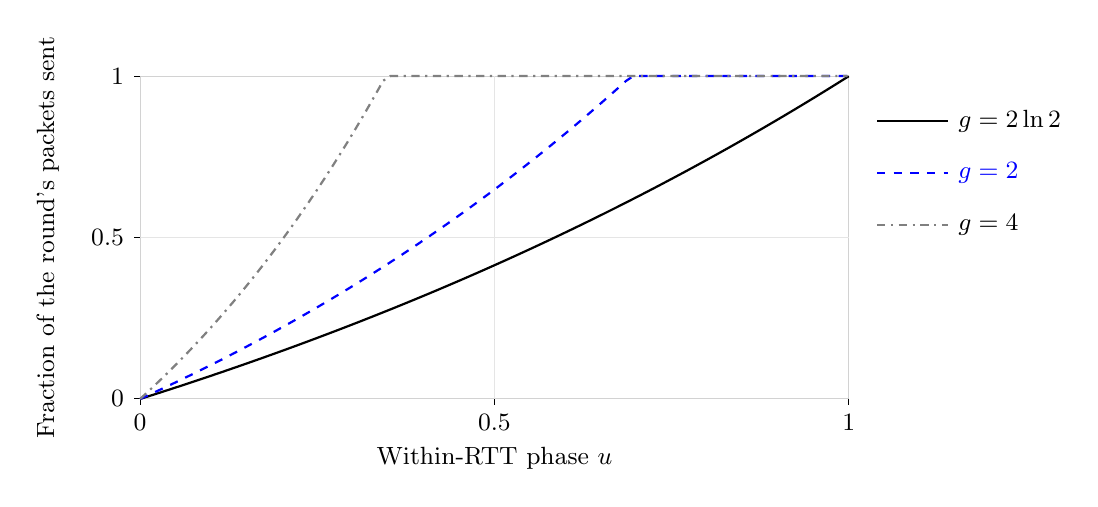
\begin{tikzpicture}[x=9cm,y=4.1cm]
 \draw[gray!35] (0,0) rectangle (1,1);
 \draw[gray!20] (0,.5)--(1,.5);
 \draw[gray!20] (.5,0)--(.5,1);
 \foreach \x/\lab in {0/0,.5/0.5,1/1}{
   \draw (\x,0)--(\x,-.018) node[below,font=\small]{\lab};}
 \foreach \y/\lab in {0/0,.5/0.5,1/1}{
   \draw (0,\y)--(-.009,\y) node[left,font=\small]{\lab};}
 \draw[thick,domain=0:1,samples=65] plot (\x,{exp(ln(2)*\x)-1});
 \draw[blue,thick,dashed,domain=0:1,samples=100] plot (\x,{min(exp(\x)-1,1)});
 \draw[gray,thick,dash dot,domain=0:1,samples=100] plot (\x,{min(exp(2*\x)-1,1)});
 \draw[thick] (1.04,.86)--(1.14,.86) node[right,font=\small] {$g=2\ln2$};
 \draw[blue,thick,dashed] (1.04,.70)--(1.14,.70) node[right,font=\small] {$g=2$};
 \draw[gray,thick,dash dot] (1.04,.54)--(1.14,.54) node[right,font=\small,text=black] {$g=4$};
 \node[below,font=\small] at (.5,-.12) {Within-RTT phase $u$};
 \node[rotate=90,font=\small] at (-.13,.5) {Fraction of the round's packets sent};
\end{tikzpicture}
\caption{Limiting send-time distributions from \eqref{eq:highcdf}, drawn
from the formula, not experimental traces. Increasing gain compresses the
sending portion of an RTT while preserving positive local packet spacing
at every finite window and gain.}\label{fig:phase}
\end{figure}

\begin{corollary}[Growth exponent and one-RTT multiplier]
For the specified scheduler and any fixed $g\ge1$,
\begin{equation}
 \boxed{\begin{aligned}
 \lim_{\tau\to\infty}\frac{\ln w_g(\tau)}{\tau}&=\min\{g/2,\ln2\},\\
 \lim_{\tau\to\infty}\frac{w_g(\tau+1)}{w_g(\tau)}&=\min\{e^{g/2},2\}.
 \end{aligned}}\label{eq:exponent}
\end{equation}
\end{corollary}
\begin{proof}
Below the threshold apply \eqref{eq:lowgrowth}. At and above it apply
\eqref{eq:phase}: the coefficient is bounded between $1/2$ and 1, and
advancing exactly one RTT preserves phase and doubles its leading term.
The uniform bounded remainder vanishes relative to that term.
\end{proof}
The physical-time growth exponent is the first limit divided by $R$.
All slow-start formulas describe an indefinitely continued growth phase.
With finite ssthresh they apply only up to the transition, not to the later
connection as $t$ tends to infinity.

\section{Gain monotonicity and the burst limit}\label{sec:limit}
For fixed packet index, increasing $g$ never delays its send. To prove this,
compare $g_2\ge g_1$ using \eqref{eq:ack}--\eqref{eq:tail}. Initially both
send packet 0 at zero and $T_0(g_2)\le T_0(g_1)$. If preceding corresponding
sends and queue tails are no later at $g_2$, the next corresponding ACK is
also no later. The maximum defining $b_k$ is no larger, and the two new
spacings are no larger. Induction proves the claim for sends and tails.
Equation~\eqref{eq:count} then gives $w_{g_2}(\tau)\ge w_{g_1}(\tau)$.
The monotonicity need not be strict, as \eqref{eq:boundary} demonstrates.

For $g\ge\gcrit$, every packet $j$ in group $m$ has
$s_j(g)=m+1+d_j/g$, with $d_j\ge0$ independent of gain. These packets have
$2^{m+1}-1\le j\le2^{m+2}-2$. Consequently, including $j=0$,
\begin{equation}
 \boxed{\lim_{g\to\infty}s_j(g)=\lfloor\log_2(j+1)\rfloor.}\label{eq:burstlimit}
\end{equation}
This is precisely the immediate-send trace: one packet at zero, two at one,
four at two, and so on. Local pacing and global concentration coexist for
finite gain; only the limit collapses each group's spacing to zero.

There is a boundary subtlety. For finite high gain,
$w_g(n)=1+2^{n-1}$, whereas the burst sender has $w_{\mathrm{burst}}(n)=2^n$.
There is no contradiction: ACKs that arrive just after $n$ for finite gain
coalesce at $n$ in the limit. Counting at a jump is not continuous under
convergence of event times. Equation~\eqref{eq:burstlimit} is a packet-time
limit, not pointwise convergence of the window at every burst jump.

\section{Extension to loss-free congestion avoidance}\label{sec:ca}
\subsection{A continuous event history across the threshold}
Take an integer threshold $\theta\ge2$ and choose the phase by the window
before the ACK:
\begin{equation}
 w_k=\begin{cases}
 w_{k-1}+1,&w_{k-1}<\theta,\\
 w_{k-1}+1/w_{k-1},&w_{k-1}\ge\theta.
 \end{cases}\label{eq:phaseupdate}
\end{equation}
The CA expression is the real-valued full-packet form of RFC 5681,
Section 3.1, equation (3), not every possible Reno byte-counting
implementation \cite{rfc5681}. For example, at $\theta=10$, ACK 9 raises
the window to 10 using SS, and ACK 10 raises it to 10.1 using CA. Flight,
the existing reservations, and the queue clock are retained at the transition.

For a real-valued window, use every available whole-packet reservation:
$F+Q=\lfloor w\rfloor$. An ACK reduces the previous count by one, so the
number of new packets is exactly
\begin{equation}
 \boxed{m_k=1+\lfloor w_k\rfloor-\lfloor w_{k-1}\rfloor.}\label{eq:mk}
\end{equation}
In CA this is one or two: the replacement packet and, when an integer window
threshold is crossed, one additional packet. Let $J_k$ be the total number
of packets ever reserved after ACK $k$, including the initial one. Then
$J_k=k+\lfloor w_k\rfloor$, and the full recurrence is
\begin{align}
 a_k&=s_{k-1}+1,& b_k&=\max\{a_k,T_{k-1}\},\\
 s_{J_{k-1}+j}&=b_k+\frac{j}{gw_k}\quad(0\le j<m_k),&
 T_k&=b_k+\frac{m_k}{gw_k}.\label{eq:carecurrence}
\end{align}
It defines the whole SS-to-CA trace without clearing outstanding packets.
With $K(\tau)=\#\{k:a_k\le\tau\}$, the exact observed window is
$\cwnd(t)=M w_{K(t/R)}$.

\subsection{Window growth indexed by ACK count}
At CA entry use a local index $j$ and initial window $u_0=a\ge1$.
Squaring $u_j=u_{j-1}+1/u_{j-1}$ gives
\begin{equation}
 \boxed{u_j^2=a^2+2j+\sum_{i=0}^{j-1}\frac1{u_i^2}.}\label{eq:casquare}
\end{equation}
Since $u_i^2\ge a^2+2i$, the sum is $O(\ln(j+1))$, and
$u_j^2=a^2+2j+O(\ln(j+1))$. This is an ACK-count result. Replacing $j$ with
$t/R$ would lose the many ACKs that can arrive within one RTT.

\subsection{A proved logarithmic term in the queue clock}
Let $k_0$ be the last SS update and define, over subsequent CA ACKs,
\begin{equation}
 \ell_k=[a_k-T_{k-1}]_+,\qquad
 \mathcal I_K=\sum_{k=k_0+1}^K\ell_k.
\end{equation}
The calligraphic $\mathcal I_K$ is cumulative waiting; it differs from the
single slow-start group wait $I_m$ of Section~\ref{sec:span}. Telescoping
\eqref{eq:carecurrence} and substituting \eqref{eq:mk} gives the exact identity
\begin{equation}
 \begin{split}
 T_K-T_{k_0}=\mathcal I_K
 +\frac1g\sum_{k=k_0+1}^K\frac1{w_k}
 +\frac1g\sum_{k=k_0+1}^K
 \frac{\lfloor w_k\rfloor-\lfloor w_{k-1}\rfloor}{w_k}.
 \end{split}\label{eq:cadecomp}
\end{equation}
The sums account respectively for replacing acknowledged packets and for
additional packets made possible by whole-MSS window growth.

\begin{theorem}[CA queue-clock asymptotic]\label{thm:ca}
For this scheduler, fixed $g\ge1$, and an indefinitely continued loss-free
CA phase,
\begin{equation}
 \boxed{T_K=\mathcal I_K+\frac1g(w_K+\ln w_K)+C+O(1/w_K),}\label{eq:catheorem}
\end{equation}
where $C$ depends on the finite initial history and fixed parameters.
\end{theorem}
\begin{proof}
The update gives the exact identity
\begin{equation}
 \frac1{w_k}=(w_k-w_{k-1})-\frac1{w_{k-1}^2w_k}.
\end{equation}
By \eqref{eq:casquare}, $w_k=\Theta(\sqrt{k})$ after the finite initial
history. The correction series therefore converges, with tail $O(K^{-1/2})
=O(1/w_K)$. The first sum in \eqref{eq:cadecomp} is
$w_K+C_1+O(1/w_K)$.

For the second sum, each sufficiently large integer threshold $n$ is crossed
exactly once. If $v_n$ is the first window at or above $n$, its preceding
value $x$ obeys $n-1<x<n$, and
\begin{equation}
 n\le v_n=x+1/x<n+\frac1{n-1}.
\end{equation}
Hence $v_n=n+O(1/n)$ and $1/v_n=1/n+O(1/n^3)$. The extra-packet sum is
$\ln w_K+C_2+O(1/w_K)$: the reciprocal-error series converges, and replacing
$\ln\lfloor w_K\rfloor$ with $\ln w_K$ changes only the stated remainder.
Substitution proves \eqref{eq:catheorem}.
\end{proof}

The logarithm here comes from additional whole packets at successive integer
window thresholds. Equation~\eqref{eq:catheorem} is a queue-clock theorem,
not yet a closed asymptotic for $\cwnd(t)$. One still needs the growth of
$\mathcal I_K$ and the relation between the queue tail and observation time.
For instance, at $g=1$ the two further estimates
\begin{equation}
 \mathcal I_K=\tfrac12\ln w_K+O(1),\qquad
 T_{K(\tau)}-\tau=O(1)\label{eq:openconditions}
\end{equation}
would imply $\tau=w+\tfrac32\ln w+O(1)$ and thus
$w(\tau)=\tau-\tfrac32\ln\tau+O(1)$. Those estimates are not proved here;
the coefficient $3/2$ is an open candidate, not a theorem of this paper.
The CA model has an increasing window and is not a statistical steady state.

\section{Relation to implementations and earlier work}\label{sec:related}
Pacing-related timing and performance effects are established topics.
Aggarwal, Savage, and Anderson analyze pacing's benefits and failures,
including feedback and synchronization effects and loss-free short-flow
latency caused by spreading transmissions \cite{aggarwal}. The premise that
pacing can delay feedback is therefore not itself a novelty claim. The
specific result here is an exact solution and comparison proof for the
declared immutable-reservation scheduler.

RFC 9002, Section 7.7, gives pacing-rate and interval examples with a gain
above one and explicitly permits different pacer architectures \cite{quic}.
The pacing Internet-Draft describes implementation choices and their
consequences \cite{pacingdraft}. These describe a broader design space than
the recurrence solved here. A nominal rate $gW/R$ does not specify whether
old deadlines are changed, whether service is reserved at admission or
transmission, or how idle intervals and batching are handled.

As a concrete versioned example, Linux v6.12's generic TCP pacing path uses
a slow-start ratio when $\cwnd<\lfloor\mathrm{ssthresh}/2\rfloor$ (both
values in segments) and the other ratio otherwise; the documented defaults are 200\% and 120\%
\cite{linux}. The threshold $2\ln2$ proved here neither derives those
engineering defaults nor proves that a smaller value is sufficient in Linux.
The actual SCP revision that motivated this study also differs: its
\texttt{scp\_output} returns while an older pacing batch remains, and its
timer can release several due packets together. It is not the per-ACK append
scheduler of Section~\ref{sec:model} \cite{scp}.

A continuously repriced fluid model would differ as well. If its active
send rate were $x(\tau)=gw(\tau)$, fixed-delay slow-start feedback would give
$w'(\tau)=gw(\tau-1)$. An exponential mode would satisfy $ze^z=g$, not
$z=g/2$. This follows directly by substitution. It is not a conflicting
solution of our packet recurrence: the fluid equation assumes immediate
realization of the current rate, whereas our old reservations keep their
intervals and timestamps. A flight-feasibility analysis would also be needed
before treating that fluid mode as an admissible sender. Results from these
different models should not be combined as if they described one scheduler.

The limits of the present results are consequently specific. Finite initial
windows other than one, delayed ACKs, variable RTT, finite link capacity,
loss recovery, and mutable reservations can change the trace. The model has
no network penalty for a large gain, so it cannot identify an optimal gain
balancing delay, loss, fairness, and throughput. Equal growth exponents also
do not establish equal finite-transfer completion times.

\section{Conclusion}
For an explicitly defined per-ACK append pacer, the transmission times admit
an exact harmonic-sum solution for every fixed gain $g\ge1$. The solution
establishes the Fibonacci comparison bound, the transition from eventual
continuous pacing to persistent RTT-separated sending intervals, and the
burst limit of individual packet timestamps. It also determines the growth
exponent and the within-RTT window trajectory, showing why those two notions
of growth must be distinguished. In congestion avoidance, exact packet
accounting isolates a logarithmic queue-clock term, while the accumulated
ACK-waiting term remains the missing part of a full physical-time asymptotic.

\appendix
\section{Proof of the Fibonacci lower comparison}\label{app:fib}
This appendix completes Theorem~\ref{thm:sandwich} without assuming that
earlier reservations necessarily produce earlier sends.

At $g=1$, equation~\eqref{eq:unity} gives
\begin{equation}
 s_0=0,\qquad s_{2k-1}=2H_k-1,\qquad
 s_{2k}=2H_k-1+\frac1{k+1}.\label{eq:fibsends}
\end{equation}
Its consecutive spacings are
\begin{equation}
 s_{j+1}-s_j=\frac1{\lfloor(j+1)/2\rfloor+1}\quad(j\ge0).
\end{equation}
For fixed-batch round $n\ge1$, put $p=f_{n+1}$, $q=f_{n+2}$. Its first
packet index is $J_n=p+q-2$, and its send times are
\begin{equation}
 \widehat s_j=n+\frac{j-J_n}{q},\qquad J_n\le j<J_n+q.
\end{equation}
Within this range the consecutive differences of $s_j-\widehat s_j$ are
the above decreasing spacings minus $1/q$. They are positive before
$j=2q-3$, zero for $j=2q-3,2q-2$, and negative afterwards. A maximum is
therefore attained at $j_*=2q-3$. This index is in the batch because
$j_*-J_n=q-p-1\ge0$ and $J_n+q-1-j_*=p\ge1$.

Substitute $j_*$ into the two send formulas to obtain
\begin{equation}
 \begin{split}
 \max_{J_n\le j<J_n+q}(s_j-\widehat s_j)
 &=2H_q-n-2+\frac{p-1}{q}=-E_n,\\
 E_n&=n+2-\frac{p-1}{q}-2H_q.
 \end{split}
\end{equation}
Initially $p=1$, $q=2$, and $E_1=0$. In the next batch the pair becomes
$(q,p+q)$. Direct subtraction gives
\begin{equation}
 E_{n+1}-E_n
 =1-\frac{q-1}{p+q}+\frac{p-1}{q}
       -2\sum_{i=1}^p\frac1{q+i}.
\end{equation}
Use the elementary identity
\begin{equation}
 \frac{q+p-i}{q(q+p)}-\frac1{q+i}
 =\frac{i(p-i)}{q(q+p)(q+i)}\ge0\quad(1\le i\le p).
\end{equation}
The sum of twice the first terms on the left is
$(p-1)/q+(p+1)/(p+q)$. Consequently,
\begin{equation}
 E_{n+1}-E_n
 =2\sum_{i=1}^p\frac{i(p-i)}{q(q+p)(q+i)}\ge0.
\end{equation}
Thus $E_n\ge0$ for all $n$, and $s_j\le\widehat s_j$ for every packet
in every batch. Packet 0 is common to both senders. Actual transmission
counts, and then ACK counts by the common delay, are therefore ordered.
Equation~\eqref{eq:count} proves $w_1(\tau)\ge w_{\mathrm{fixed}}(\tau)$
at every time. Section~\ref{sec:limit} extends this to $g\ge1$, and the
fixed-batch boundary values \eqref{eq:fib} finish the proof.

\begin{thebibliography}{9}
\raggedright
\bibitem{rfc5681}
M. Allman, V. Paxson, and E. Blanton.
\emph{TCP Congestion Control}. RFC 5681, September 2009.
\url{https://www.rfc-editor.org/rfc/rfc5681}.

\bibitem{aggarwal}
A. Aggarwal, S. Savage, and T. Anderson.
Understanding the Performance of TCP Pacing.
\emph{IEEE INFOCOM}, pp. 1157--1165, 2000.
\url{https://cseweb.ucsd.edu/~savage/papers/Infocom2000pacing.pdf}.

\bibitem{quic}
J. Iyengar and I. Swett.
\emph{QUIC Loss Detection and Congestion Control}. RFC 9002, May 2021.
\url{https://www.rfc-editor.org/rfc/rfc9002}.

\bibitem{pacingdraft}
M. Welzl, W. Eddy, V. Goel, and M. T\"uxen.
\emph{Pacing in Transport Protocols}.
\texttt{draft-irtf-iccrg-pacing-02}, June 26, 2026. Work in progress;
this citation fixes the version discussed.
\url{https://datatracker.ietf.org/doc/html/draft-irtf-iccrg-pacing-02}.

\bibitem{linux}
Linux v6.12. \texttt{tcp\_update\_pacing\_rate} and TCP pacing ratio
documentation.
\href{https://github.com/torvalds/linux/blob/v6.12/net/ipv4/tcp_input.c}{Versioned source};
\href{https://docs.kernel.org/6.12/networking/ip-sysctl.html}{parameter documentation}.

\bibitem{scp}
Skai Uijing. SCP source, \texttt{scp.c},
\href{https://github.com/skaiui2/SCP/tree/bf9d8873b0f8815073f661b4606b7de4bd9bed71}{revision \texttt{bf9d8873b0f8}}.
\end{thebibliography}
\end{document}
